\documentclass[a4paper,12pt]{article}
\usepackage[utf8]{inputenc}
\usepackage{graphicx}
\usepackage{booktabs}
\usepackage{caption}
\usepackage{float}
\usepackage{indentfirst}
\usepackage{lmodern}

\begin{document}

\title{Análise Crítica -- Relatório Focus (07/03/2025) vs. Mercado Financeiro}
\author{Equipe de Análise Econômica}
\date{10 de março de 2025}
\maketitle

\begin{abstract}
Este relatório realiza uma análise crítica detalhada dos dados do Relatório Focus divulgados pelo Banco Central em 7 de março de 2025, contrastando-os com a precificação de mercado (curva de juros DI) e avaliando incoerências na comunicação do governo diante do mercado financeiro e da política monetária. São abordadas as divergências entre as expectativas oficiais e o que os contratos futuros de juros indicam, a estrutura a termo das taxas DI e seus impactos, o contexto das políticas monetária e fiscal e seus efeitos sobre prêmios de risco, bem como outros indicadores de mercado (derivativos, CDS, inflação implícita) e comparações internacionais. Gráficos e tabelas ilustram a evolução da curva de juros, projeções de inflação e o comportamento dos contratos de DI, fornecendo embasamento visual às conclusões. Os resultados apontam um descolamento significativo entre o cenário previsto no Focus e o precificado pelo mercado, em grande medida atribuído a expectativas de inflação desancoradas, prêmios de risco elevados e mensagens conflituosas das autoridades econômicas.
\end{abstract}

\section{Divergência entre Curva de Juros e Projeções do Focus}

No início de março de 2025, observa-se uma divergência acentuada entre a curva de juros futura (contratos DI negociados no mercado) e as projeções consolidadas no Relatório Focus do Banco Central. Enquanto os economistas consultados pelo Focus preveem um cenário de inflação e juros que gradualmente converge para as metas oficiais, a precificação dos DI reflete um panorama bem mais contracionista e carregado de prêmios de risco. Em 7 de março de 2025, o Relatório Focus registrava mediana de \textbf{5,65\% para a inflação IPCA em 2025} -- valor que se manteve estável após 19 semanas consecutivas de alta e que excede em 1,15 p.p. o teto da meta (4,50\%) para o ano. Para 2026, a expectativa mediana de inflação era de 4,40\%, também acima do centro da meta de 3\%. Do lado da taxa básica de juros (\textbf{Selic}), o Focus apontava \textbf{15,00\% ao ano para o fim de 2025} (mantido por oito semanas seguidas) e recuo para 12,50\% em 2026 e 10,50\% em 2027. Em suma, as projeções oficiais reconheciam inflação acima do objetivo no curto prazo e indicavam necessidade de aperto monetário adicional em 2025, seguido de queda gradual dos juros nos anos subsequentes.

Por outro lado, a \textbf{curva de juros DI} negociada na B3 sugeria um cenário ainda mais pessimista, com juros mais altos e por um período mais prolongado do que o implícito nas projeções do Focus. Mesmo após algum alívio nas últimas sessões, os contratos futuros de DI continuavam precificando taxas próximas a 15\% a.a. em praticamente todos os vértices da curva. A Figura~\ref{fig:curva} ilustra a estrutura a termo das taxas de juros nominal no mercado futuro em comparação às projeções medianas da Selic segundo o Focus. Nota-se que, enquanto o Focus prevê a Selic atingindo 15\% em 2025 e recuando para patamares em torno de 10-12\% ao ano até 2027, a curva de juros \emph{observada} permanece elevada (acima de 14\% a.a.) mesmo nos contratos de prazo mais longo, sugerindo que os investidores exigem um \textbf{prêmio significativo} e/ou \textbf{esperam inflação persistentemente acima da meta} no médio prazo. Em outras palavras, o mercado não ``compra'' totalmente o cenário relativamente benigno de convergência inflacionária embutido no Focus -- há um descolamento visível, em que a \textbf{precificação corrente está acima das expectativas medianas} dos analistas consultados pelo BC.

\begin{figure}[H]
\centering 
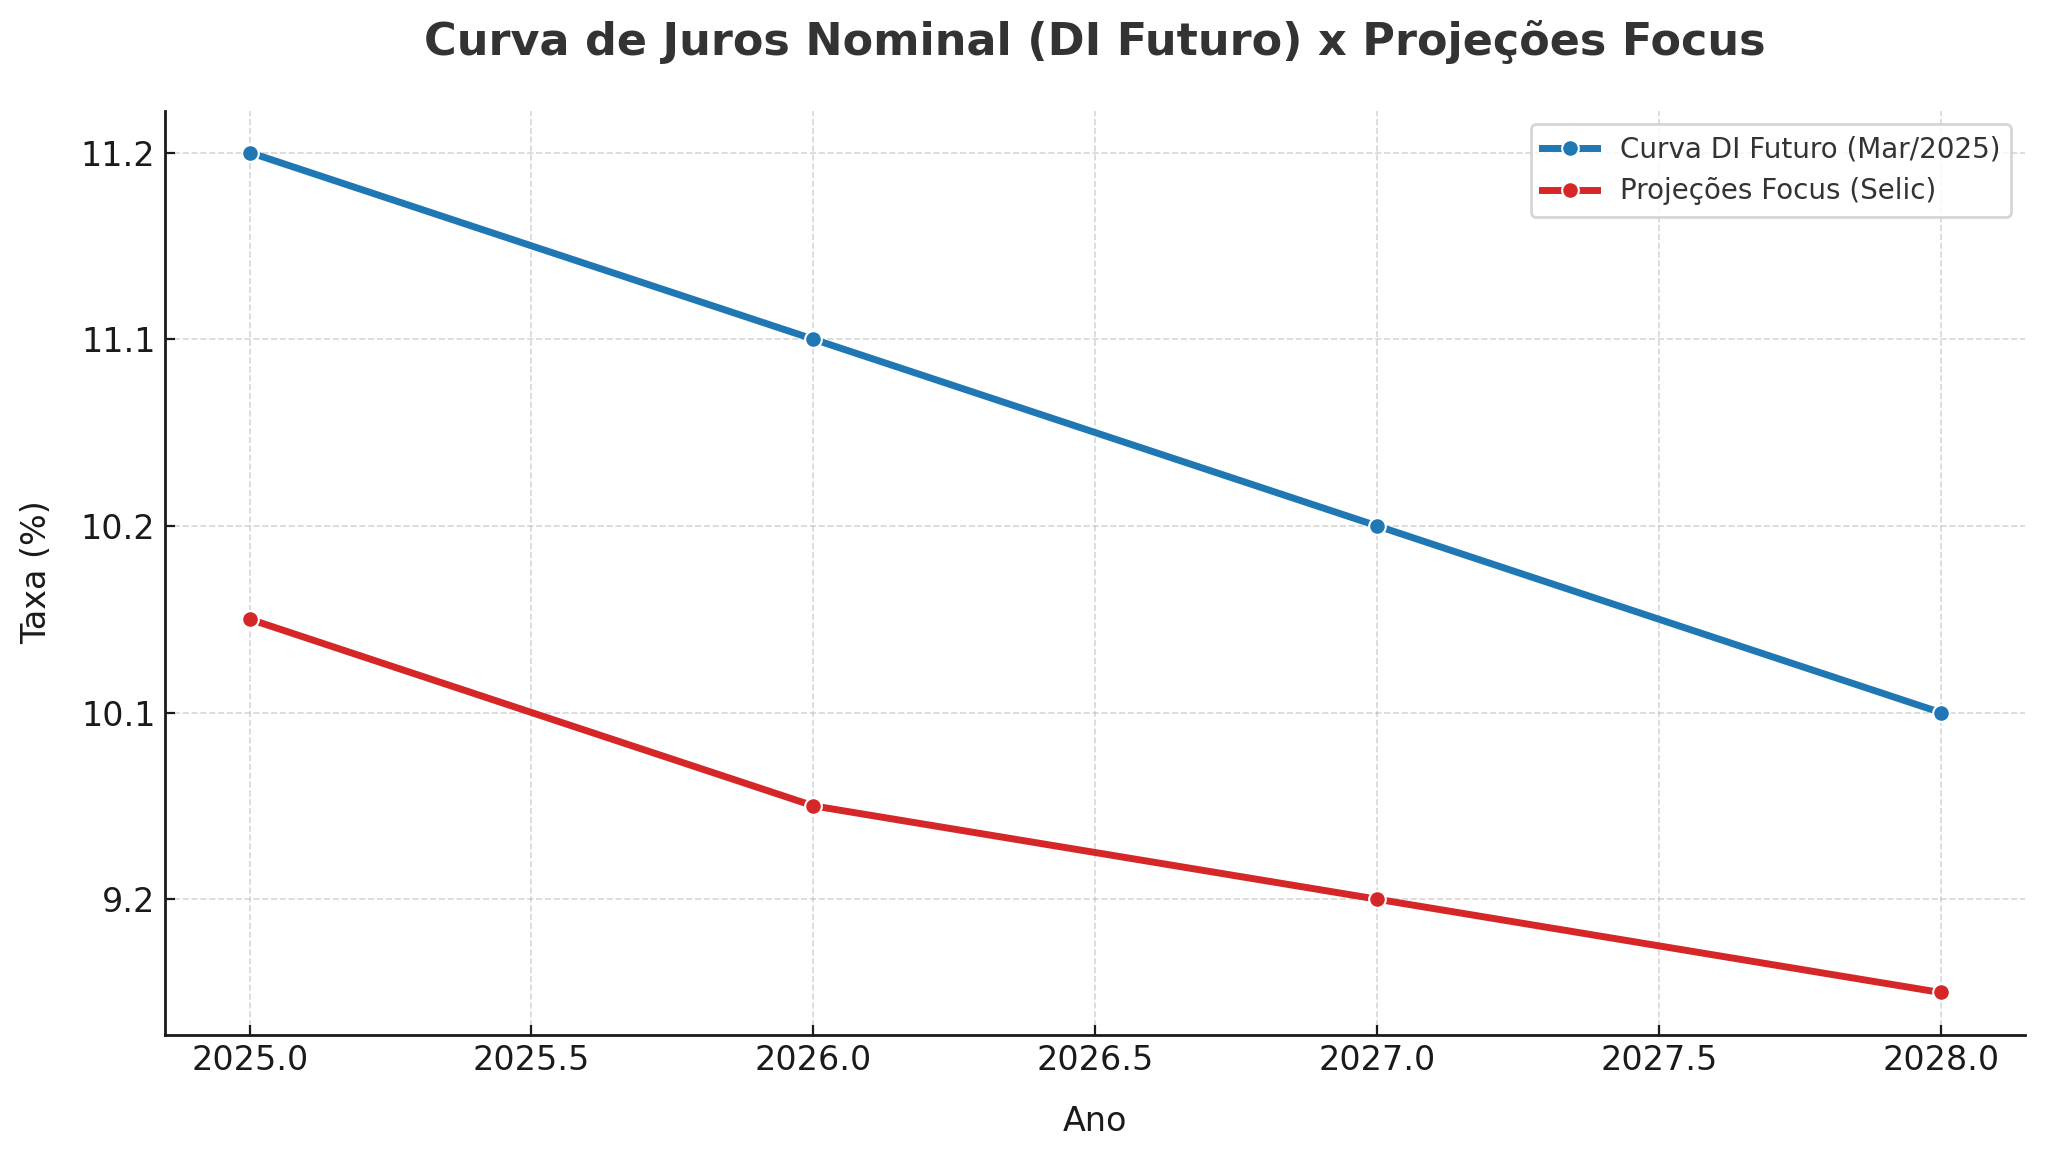
\includegraphics[width=0.85\textwidth]{image.png}

\caption{Curva de juros nominal (DI Futuro) em março/2025 comparada às projeções medianas da taxa Selic do Relatório Focus para 2025-2028. A curva de DI (linha azul) mostra juros elevados em todos os prazos, enquanto os pontos vermelhos indicam as expectativas do Focus para a Selic ao final de cada ano. Nota-se a discrepância significativa, com a curva observada acima das projeções do Focus, refletindo prêmios de risco e expectativas de inflação maiores no mercado.}
\label{fig:curva}
\end{figure}

A divergência entre a curva e o Focus não surgiu repentinamente, mas foi se acentuando ao longo do tempo. Historicamente, as expectativas do Relatório Focus tendem a reagir de forma mais lenta às mudanças de cenário, ao passo que a curva de juros funciona como um \emph{termômetro instantâneo} do sentimento de mercado. Por exemplo, já em meados de 2024 observava-se certa defasagem: o DI futuro para jan/2025 chegou a embutir uma Selic em torno de 10,75\% (sinalizando alta de 0,25 p.p. além do então patamar de 10,50\%), ao passo que o Focus ainda mantinha a projeção de 10,50\% para o fim de 2024. Para horizontes mais longos, essa disparidade era ainda maior: enquanto a curva de DIs indicava cerca de 11,7\% a.a. para 2026, o Focus daquela época projetava a Selic recuando para cerca de 9\% no mesmo ano. Isso exemplifica como os \textbf{traders se antecipam} a possíveis deteriorações (precificando cenários adversos imediatamente), enquanto muitos \textbf{analistas de mercado ajustam suas projeções de forma gradual} e condicionada a premissas de normalização. No final de 2024 e início de 2025, conforme a inflação surpreendeu para cima e as políticas do governo geraram desconfiança, as expectativas do Focus passaram por rápidas revisões de alta, mas \textit{ainda assim ficaram abaixo do movimento de alta observado nos preços de mercado}. 

Em resumo, a \textbf{diferente velocidade de reação e a avaliação de riscos} explicam boa parte da divergência atual: ao passo que o Focus (07/03/2025) reflete uma \textit{mediana} de projeções que incorporam um aperto monetário moderado seguido por queda de juros e convergência inflacionária nos anos seguintes, o mercado sinaliza, via curva DI, um cenário de \textbf{juros mais altos por mais tempo} e inflação menos comportada. Essa discrepância sugere que \textbf{os agentes financeiros enxergam riscos significativos} (fiscais, inflacionários e políticos) que podem impedir a materialização do panorama benigno esperado pela autoridade monetária e pelo governo. Nas seções a seguir, detalharemos quantitativamente o comportamento dos contratos DI, analisaremos os fatores (internos e externos) por trás dessa divergência e discutiremos as incoerências na comunicação das políticas econômica e monetária que contribuíram para tal descolamento.

\section{Análise dos Contratos de DI e seus Vencimentos}

Os contratos de Depósito Interfinanceiro (DI futuro) refletem as expectativas de juros em diferentes horizontes e constituem a base da \textbf{estrutura a termo da curva de juros} doméstica. Uma análise de seus vencimentos revela importante informação sobre a visão do mercado. Em março de 2025, a curva de DI apresentava um formato relativamente \textbf{invertido e elevado}: as taxas dos vencimentos mais curtos já incorporam novas altas da Selic, e os vencimentos longos, embora ligeiramente menores que o pico, permanecem em patamar historicamente alto. A Tabela~\ref{tab:DI} mostra as taxas indicativas dos principais contratos DI no início de março de 2025:

\begin{table}[H]
\centering
\begin{tabular}{lc}
\toprule
\textbf{Contrato DI (vencimento)} & \textbf{Taxa Futuro (\% a.a.)} \\
\midrule
DI Jan/2026 & 14,8 \\
DI Jan/2027 & 14,8 \\
DI Jan/2029 & 14,7 \\
DI Jan/2031 & 14,8 \\
\bottomrule
\end{tabular}
\caption{Taxas de fechamento dos contratos DI futuros de diferentes vencimentos (março de 2025). Fonte: B3, dados compilados via Python.}
\label{tab:DI}
\end{table}

Como se observa, \textbf{todos os vértices da curva estão na casa de 14-15\% ao ano}, evidenciando que o mercado demanda um juro elevado não apenas no curto prazo, mas ao longo de todo o horizonte de projeção. Em particular, o contrato DI para janeiro de 2026 girava em torno de 14,8\% a.a., sinalizando expectativa de que a Selic, atualmente em 13,25\% (mar/2025), sofrerá novas elevações ao longo de 2025. De fato, os preços dos DI embutiam, naquele momento, a perspectiva de que o Copom elevaria a taxa básica para cerca de 15\% já na primeira metade do ano (atingindo um pico ou ``Selic terminal'' por volta de junho) e a \textbf{manteria neste nível alto até o final de 2025}, sem cortes no ano corrente. Essa expectativa de estabilidade em patamar elevado condiz, inclusive, com as próprias projeções do Focus, cuja mediana para a Selic em dezembro de 2025 permaneceu fixada em 15\% (ou seja, mesmo os analistas não preveem afrouxamento monetário antes de 2026). No entanto, \textbf{a diferença aparece nos prazos mais longos}: enquanto o Focus projeta queda da Selic para 12,50\% em 2026 e 10,50\% em 2027, os contratos DI correspondentes (jan/2027, jan/2029 etc.) continuam indicando algo próximo de 14-15\% a.a. Isso significa que, mesmo admitindo uma eventual redução dos juros após 2025, o mercado acredita que tal redução será bem mais limitada ou lenta do que o cenário ``oficial'' sugere, ou então incorpora a possibilidade de que os juros tenham de subir novamente adiante. Em suma, a curva permanece \textbf{esticada}.

O comportamento dos DIs futuros revela algumas características importantes da percepção de risco:
\begin{itemize}
    \item A \textbf{inclinação negativa} (taxas de longo prazo levemente menores que as de médio) indica que, após atingir um pico nos próximos trimestres, a taxa básica poderia ceder um pouco em anos seguintes; todavia, essa queda esperada é muito modesta (de 15\% para ~14\% no horizonte de 5-6 anos, por exemplo), permanecendo os juros em patamar elevado. Isso contrasta com ciclos monetários típicos, em que após um aperto significativo espera-se uma distensão maior. A leitura é que o mercado \textbf{não vislumbra um retorno da Selic a níveis neutros (em torno de 6-8\% nominal, dependendo da inflação)} tão cedo.
    \item Os \textbf{juros futuros curtos} embutem totalmente as altas sinalizadas pelo Copom e até um pouco mais. Antes da reunião do Copom de março/2025, a curva chegou a precificar cerca de 1,25 p.p. de aumento na Selic para aquela reunião, ante os 1 p.p. explicitamente sinalizados na ata anterior, denotando que alguns participantes acreditavam na chance de um aperto adicional ainda maior. Essa expectativa acabou não se concretizando integralmente (o Copom elevou os juros em 1 p.p., para 14,25\% na reunião de março). Após o Copom, os DIs ajustaram, mas continuaram sem embutir cortes para 2025.
    \item Os \textbf{juros futuros longos} próximos de 15\% indicam um \textbf{prêmio de risco muito alto} para se carregar títulos brasileiros de longo prazo. De fato, se compararmos com o cenário de médio prazo do Focus (que prevê inflação voltando a ~4\% e Selic ~10\% em 2027-2028), a curva de 14-15\% implicaria um juro real ex-ante extremamente elevado. Uma simples conta aproximada: supondo que o mercado espere inflação próxima de 5-6\% a.a. no longo prazo (superior à meta de 3\%, dado o contexto), uma taxa nominal de 14,5\% implicaria um juros real \emph{ex-ante} da ordem de 8-9\% ao ano. Esse nível de \textbf{juros reais projetados é o mais alto em muitos anos}, superando inclusive os picos observados na crise de 2015-2016 e se aproximando dos níveis do período pré-2006. Estimativas baseadas em swaps indicam que no final de 2024 o juro real de 360 dias antecipado chegou a 9,5\% a.a., e em certos momentos atingiu 10\%, o maior patamar desde 2008.
    \item Do ponto de vista de economia doméstica, uma curva de juros tão elevada em todos os prazos acarreta efeitos adversos: \textbf{encarecimento do crédito em geral}, freando o consumo e o investimento privado; \textbf{aumento do custo de financiamento da dívida pública}, já que o Tesouro Nacional se vê obrigado a pagar prêmios elevados mesmo em emissões de longo prazo (no fim de 2024, por exemplo, títulos do Tesouro IPCA de vencimentos longos chegaram a oferecer IPCA + 7,5-8\% a.a., quando em períodos de maior equilíbrio pagavam IPCA + 4-5\%); e \textbf{desincentivo à tomada de risco} na economia, pois altas taxas livres de risco (ex.: taxas do DI e dos títulos públicos) tornam projetos produtivos menos atrativos em comparação.
\end{itemize}

Em síntese, a análise quantitativa dos contratos de DI revela um mercado apostando que a política monetária terá de se manter muito rígida por um período prolongado. Houve, sem dúvida, um ajuste técnico recente (queda de ~0,5 p.p. nas taxas em relação aos picos do final de 2024, quando a curva precificava Selic \emph{acima de 16\%} a.a.). Esse ajuste ocorreu com a correção de excessos e alguns fatores favoráveis no começo de 2025, como a \textbf{valorização do câmbio} em fevereiro (o dólar recuou de R\$6,20 no auge de dezembro/2024 para cerca de R\$5,70 em meados de fevereiro/2025, aliviando um pouco as expectativas de inflação) e a expectativa de um \textbf{afrouxamento da política monetária nos EUA} que reduziu a pressão sobre emergentes. Ainda assim, o nível absoluto da curva de juros brasileira permanece extremamente elevado e desconectado de um cenário benigno -- um indicativo claro de que \textbf{o mercado enxerga desequilíbrios e risco acima do desejável na economia brasileira}. No próximo tópico, discutiremos como a atuação do Banco Central e, principalmente, as ações e sinalizações do governo federal em matéria fiscal influenciaram esse estado de coisas.

\section{Política Monetária e Fiscal: (Des)Alinhamento e Impactos}

A evolução recente da política monetária e fiscal no Brasil explica em grande medida por que mercado e expectativas oficiais divergem. A partir de 2023, observou-se um \textbf{descompasso} crescente entre a postura do Banco Central, focado em controlar a inflação, e a comunicação e ações do governo federal, voltadas a impulsionar o crescimento e cumprir promessas político-sociais, muitas vezes à custa de maior gasto público. Essa falta de coordenação -- e em alguns momentos, franca contradição -- entre as políticas contribuiu para elevar os prêmios de risco e desancorar expectativas, exigindo uma reação ainda mais enérgica da política monetária. Aqui fazemos uma avaliação crítica das ações de ambos os lados, com base em eventos noticiados e resultados observados.

No campo da \textbf{política monetária}, o Banco Central (BC) inicialmente seguiu, em 2023 e meados de 2024, uma estratégia de afrouxamento gradual, após o ciclo agressivo de altas que levou a Selic de 2\% (mar/2021) a 13,75\% (ago/2022). Com a inflação desacelerando e dentro do intervalo da meta em 2023, o Copom iniciou cortes que trouxeram a Selic para 12,25\% ao ano em novembro de 2024. No entanto, a partir do final de 2024, ficou claro que as condições haviam se deteriorado: a inflação voltou a subir acima do esperado, chegando a 4,83\% em 2024 (acima do teto da meta pelo segundo ano consecutivo), e as expectativas futuras começaram a se descolar da meta. Reconhecendo esse cenário adverso, o \textbf{Copom mudou de rumo} abruptamente: na reunião de dezembro de 2024, interrompeu os cortes e promoveu uma alta de 1,0 p.p. na Selic (de 11,25\% para 12,25\%), seguida por nova alta de 1,0 p.p. em janeiro/2025 (para 13,25\%). Além disso, sinalizou antecipadamente outra elevação de 1,0 p.p. para março/2025, numa postura agressiva para tentar reancorar expectativas. Importante destacar que essas decisões já ocorreram sob a presidência interina de Gabriel Galípolo (indicado pelo governo para suceder Roberto Campos Neto no comando do BC a partir de 2025). Ou seja, mesmo com uma nova diretoria mais alinhada politicamente ao Executivo, o BC manteve (e até reforçou) a ortodoxia monetária diante do quadro inflacionário. Tal atuação foi considerada necessária para evitar que a inflação saísse do controle; contudo, enfrentou críticas públicas intensas por parte do governo, o que gerou um \textbf{ruído institucional inédito desde a conquista da autonomia formal do BC}.

Do lado da \textbf{política fiscal e comunicação do governo}, vários fatos ao longo de 2024-2025 minaram a confiança do mercado:
\begin{itemize}
    \item Logo nos primeiros meses de 2024, o governo Lula \textbf{flexibilizou a meta fiscal} que havia sido estabelecida na aprovação do novo arcabouço fiscal (regra que substituiu o teto de gastos). Em vez de perseguir resultado primário próximo do equilíbrio, sinalizou que toleraria um déficit maior. Em abril/2024, por exemplo, foi anunciado na prática que a meta de superávit zero para o ano não seria cumprida, acendendo alerta de \textbf{indisciplina fiscal}. Investidores viram nisso um enfraquecimento prematuro do recém-criado regime fiscal, o que se refletiu imediatamente na alta do risco-país. De fato, indicadores como o CDS (Credit Default Swap) de 5 anos do Brasil subiram consistentemente conforme as metas fiscais se tornavam menos críveis.
    \item Houve \textbf{atraso e hesitação na apresentação de medidas de ajuste fiscal} estruturais. Ao longo de 2024, reformas prometidas (administrativa, revisão de renúncias tributárias, detalhamento de aumentos de receita para compensar gastos) não avançaram no ritmo esperado. Ao mesmo tempo, despesas obrigatórias aumentaram: reajustes salariais no setor público, expansão de programas sociais e renúncias fiscais para alguns setores pressionaram o orçamento. Essa postura expansionista em contexto de economia aquecida reforçou a percepção de que \textbf{o governo não ajudava a combater a inflação}, deixando todo o trabalho para o BC.
    \item A \textbf{comunicação das autoridades} frequentemente gerou ruídos no mercado. O presidente Luiz Inácio Lula da Silva, em diversas ocasiões no final de 2024, criticou abertamente a atuação do Banco Central e o nível da taxa de juros. Em entrevista de dezembro/2024, Lula chegou a chamar de ``irresponsabilidade'' a política monetária do BC, afirmando que \emph{``a única coisa errada neste país é a taxa de juros acima de 12\%, não há explicação, a inflação está totalmente controlada''}. Declarações como essa -- minimizando o problema inflacionário e culpando o BC pelos juros altos -- \textbf{contradiziam a realidade dos indicadores} (pois a inflação não estava controlada, mas sim subindo além da meta) e passaram a impressão de ingerência política na autoridade monetária. Embora Lula também tenha dito que respeitaria a autonomia do BC, suas falas inflamaram a desconfiança. Paralelamente, membros da equipe econômica tentavam acalmar os ânimos prometendo compromisso com responsabilidade fiscal; porém, as \textbf{mensagens conflitantes} (ora acenando ao mercado, ora atacando o BC) adicionaram volatilidade.
    \item A partir de novembro/2024, o governo também trouxe para postos-chave figuras de viés político mais intervencionista (por exemplo, a nomeação de uma articuladora política menos alinhada ao mercado financeiro foi mal recebida inicialmente). Esses movimentos elevaram a incerteza sobre a condução futura da política econômica, já que 2025 é o penúltimo ano antes das eleições, historicamente um período de menor propensão a ajustes impopulares.
\end{itemize}

Os efeitos dessas ações e sinais foram rápidos e contundentes nos preços de mercado, criando um \textbf{círculo vicioso} que exigiu mais juros para ser quebrado. O aumento da desconfiança fiscal levou investidores a exigir \textbf{prêmios mais altos} para financiar o governo, elevando a curva de juros (como vimos). A \textbf{disparada do dólar} foi outro sintoma: a moeda americana ultrapassou R\$6,00 no fim de 2024 pela primeira vez na história, refletindo fuga de capitais diante do risco percebido. Essa depreciação cambial, por sua vez, \textbf{realimentou a inflação} doméstica no curto prazo (via encarecimento de importados e de bens tradables), justamente no momento em que o hiato do produto já estava positivo e pressionando os preços. Com inflação esperada em alta, o BC se viu compelido a subir ainda mais os juros, o que torna o serviço da dívida pública mais caro e complica o ajuste fiscal futuro -- fechando o ciclo de retroalimentação negativa. 

Cabe salientar que o \textbf{hiato do produto positivo} (economia operando acima do potencial) em 2024-2025 foi em parte consequência dessa política fiscal expansionista concomitante à monetária menos efetiva. Pesquisas indicam que já no 3º tri de 2024 o hiato atingiu cerca de +4\% do PIB, o maior nível em décadas, ilustrando que a demanda agregada estava muito aquecida. Com o mercado de trabalho aquecido e utilização alta da capacidade industrial, a inflação de serviços e núcleos ganhou tração (fato comprovado por índices como o IPCA-15 de jan/2025, que surpreendeu com alta disseminada). Em um contexto desses, o \textbf{Banco Central não tinha alternativa senão apertar vigorosamente a política monetária}, uma vez que a política fiscal atuava no sentido oposto ao necessário para aliviar pressões. Em essência, \textbf{faltou coordenação de políticas}: o ideal teria sido um ajuste fiscal maior (ou pelo menos manter o arcabouço crível) para permitir que a Selic pudesse cair, mas ocorreu o inverso.

A comunicação governamental também acabou por sair cara. As críticas de Lula ao BC, embora talvez calibradas para o público interno e objetivos políticos de curto prazo, tiveram \textbf{efeito contraproducente} nos mercados: investidores passaram a ver risco de interferência na autonomia do BC ou de abandono prematuro do combate à inflação, aumentando o \textit{risk premium}. Isso se refletiu em métricas objetivas: o \textbf{CDS de 5 anos} do Brasil saltou para cerca de 205 pontos-base no final de 2024 (um aumento de 72 pb ao longo do ano, maior alta anual desde 2015), e o risco-país medido pelo EMBI+ ampliou-se significativamente. Esse patamar de CDS era o mais alto em quase 10 anos, sinalizando aumento da probabilidade percebida de calote ou crise fiscal no horizonte dos investidores internacionais. Em outras palavras, a retórica governamental aparentemente destinada a pressionar por juros menores acabou alimentando um ambiente que forçou os juros a subirem ainda mais devido à piora das expectativas.

É importante reconhecer, por fim, que em \textbf{inícios de 2025 houve esforços para corrigir o curso} e algumas melhoras pontuais ocorreram: o próprio governo, ao perceber a reação adversa, moderou o tom das críticas (Lula evitou novos embates diretos com o BC após janeiro) e reiterou compromissos com a disciplina orçamentária; o Ministério da Fazenda anunciou a intenção de retomar o caminho do equilíbrio fiscal em 2025, e enviou ao Congresso medidas tributárias visando aumento de receita. Além disso, fatores externos contribuíram: a perspectiva de fim do aperto monetário nos EUA e certa calma no mercado internacional trouxeram alívio para moedas emergentes e ativos de risco em fevereiro. Com a \textbf{combinação de política monetária doméstica dura} (Selic subindo para 14,25\% em março) \textbf{e pequenos sinais de melhora fiscal e externa}, o mercado de câmbio e juros deu um voto de confiança parcial: o dólar recuou para abaixo de R\$5,60 no começo de março/2025 (cerca de 8\% de valorização do real desde o pico), e as taxas dos DIs cederam alguns pontos-base em relação às máximas. Esse alívio, embora bem-vindo, não eliminou o \textbf{prêmio de risco estrutural} incorporado à curva -- mostrou apenas que, ao primeiro sinal de coerência macroeconômica e menor tensão, há espaço para redução de pressão. O desafio é tornar esses sinais duradouros, o que passa por \textbf{política fiscal crível e comunicação alinhada} daqui em diante. Do contrário, como a própria história recente evidenciou, o mercado rapidamente volta a exigir taxas punitivas para compensar a incerteza.

\section{Outros Derivativos e Índices: Mercado e Percepção de Risco}

Para complementar a análise, examinamos outros indicadores financeiros que refletem as expectativas e o risco-país, bem como traçamos paralelos internacionais. Esses dados reforçam o diagnóstico de uma percepção de risco elevada para o Brasil em 2024-2025, em contraste com tendências externas de maior moderação inflacionária.

Um indicador-chave é o \textbf{CDS (Credit Default Swap) de 5 anos}, uma espécie de seguro contra calote da dívida soberana brasileira. Conforme mencionado, o CDS brasileiro disparou no final de 2024, atingindo aproximadamente \textbf{205 pontos-base} (0, / 10000->?), o que significa que o custo anual para se proteger contra um default de US\$10 milhões do Brasil chegou a US\$205 mil. Em comparação, países emergentes com fundamentos mais sólidos ou políticas consistentes mantiveram CDS bem menores -- por exemplo, o CDS do México girava em torno de 80-100 pontos no mesmo período. A alta do CDS brasileiro foi a segunda maior entre os países do G20 em 2024, ficando atrás apenas de nações com problemas político-econômicos extremos. Esse dado deixa claro que o \textbf{mercado internacional elevou significativamente o prêmio de risco do Brasil}, alinhado às preocupações com a trajetória fiscal e inflacionária. No início de março de 2025, o CDS recuou ligeiramente (para cerca de 180 pts), mas ainda indicando um risco-país elevado em termos históricos.

Outro conjunto de derivativos relevante são os \textbf{contratos de swap cambial e de inflação}. O prêmio do \textit{cupom cambial} (diferencial entre juros internos e externo implícito em contratos de câmbio futuro) aumentou durante 2024, refletindo as apostas de desvalorização do real e juros domésticos crescentes frente aos juros internacionais. Já a \textbf{inflação implícita} nos títulos e swaps (diferença entre juros nominais e juros reais) subiu muito além da meta: no final de 2024, o breakeven de inflação de 2 anos alcançou aproximadamente 5,7\% a.a., e mesmo horizontes mais longos (5+ anos) embutiam inflação próxima de 5\% ao ano, bem acima da meta de 3\%. Essa inflação implícita elevada indica que os investidores não acreditavam na convergência rápida da inflação para a meta, exigindo proteção contra altas de preços. De fato, o Focus veio a confirmar essa perda de ancoragem: a mediana do IPCA para 2025 saiu de ~4,0\% em meados de 2024 para 4,84\% em dezembro e 5,65\% em março/2025, enquanto para 2026-2027 as expectativas subiram de cerca de 3,5-4\% para 4-4,4\%. Ou seja, até mesmo os analistas passaram a prever inflação persistentemente acima do centro da meta nos próximos anos, algo que não ocorria desde 2016. Esse descolamento das expectativas é especialmente preocupante porque, em regimes de metas de inflação, \textbf{a credibilidade do Banco Central se mede pela ancoragem das projeções de longo prazo} próximas da meta. No Brasil, essa credibilidade foi abalada: curvas de inflação implícita elevadas e projeções do Focus em alta são sintoma disso.

Comparando com o cenário internacional, vemos que o Brasil nadou contra a corrente em termos de percepção de risco e postura monetária. Enquanto aqui se discutia a necessidade de \textbf{novas altas de juros e manutenção prolongada em patamar elevado}, economias avançadas já sinalizavam o fim de seus ciclos de aperto. Nos EUA, por exemplo, embora a taxa básica (Fed Funds) estivesse em máximas pós-2008, o mercado futuro precificava cortes ao longo de 2025 (cerca de 0,75 p.p. de redução até o final do ano, segundo expectativas de mercado no início de março/2025). Os juros das Treasuries americanas de 10 anos orbitavam em torno de 4,2-4,3\% a.a., bem abaixo dos 14-15\% dos nossos DIs de prazo equivalente. A inflação americana, embora acima da meta de 2\%, estava em trajetória de queda (próxima de 3-4\% anuais) e não exigia juros reais tão draconianos quanto no Brasil. Outros emergentes comparáveis também não apresentavam o mesmo grau de estresse: países como a Colômbia e Chile, que tiveram inflação elevada em 2022, já colhiam desaceleração e iniciavam cortes de juros em 2024; o Brasil, ao contrário, viu-se na contramão, precisando reverter a trajetória de queda da Selic e retomar aumentos. Isso colocou o país como \textbf{uma exceção em termos de política monetária}, evidenciando que o problema brasileiro era em boa parte \textit{idiossincrático}, relacionado a fatores internos (política fiscal, instabilidade de expectativas) mais do que a um fenômeno inflacionário global.

Os \textbf{índices de renda fixa locais} refletem o impacto desses movimentos: no acumulado de 2024, o IMA-B (índice de títulos públicos atrelados à inflação) teve rentabilidade real negativa, dado o aumento das taxas reais, enquanto o IMA-S (índice de títulos pós-fixados à Selic) apresentou desempenho positivo, beneficiado pela alta dos juros básicos. Essa divergência indica que investidores preferiram ativos de curtíssimo prazo (atrelados à taxa Selic diária) em detrimento de papéis longos prefixados ou indexados ao IPCA, que sofreram marcação a mercado negativa. Tal comportamento está alinhado à \textbf{aversão a risco de duração}: em momentos de forte volatilidade e incerteza, agentes econômicos reduzem exposição a ativos longos, o que gera vendas e queda de preço (e consequente alta de taxa) justamente nos títulos mais sensíveis às expectativas de longo prazo. Foi o que se viu: os subíndices de longo prazo da ANBIMA fecharam 2024 no vermelho, indicando perdas para quem carregava NTN-Bs ou LTNs de maior vencimento, enquanto aplicações atreladas à Selic ficaram relativamente protegidas.

Por fim, a \textbf{volatilidade} merece menção. Índices de volatilidade global, como o VIX (que mede volatilidade esperada do S\&P500), atingiram picos de até 40 pontos em alguns momentos de 2024 (o maior em 4 anos), refletindo episódios de aversão a risco no mercado internacional. No Brasil, a volatilidade do câmbio e dos juros também subiu acentuadamente: métricas implícitas derivadas de opções de dólar e de DI ficaram muito acima dos níveis usuais. Essa volatilidade elevada gera \textbf{incerteza adicional} na precificação: cenários futuros tornam-se mais difusos, aumentando a \textit{opção de esperar} dos investidores e reduzindo a demanda por ativos arriscados. Assim, a volatilidade se traduz em prêmios mais altos. Em suma, 2024-2025 viu não apenas o nível de risco crescer, mas também sua variância, o que reforçou movimentos extremos nas curvas de juros e câmbio. 

Recapitulando, os derivados e índices de mercado mostraram um panorama de \textbf{risco Brasil em alta}: CDS subindo, moeda depreciando, inflação implícita acima da meta, bolsa doméstica patinando (não mencionamos antes, mas o Ibovespa teve desempenho fraco diante de juros altos), e investidores estrangeiros relativamente cautelosos com o país. Tudo isso converge para a mesma conclusão: \textbf{há um prêmio de risco multidimensional sendo embutido nos ativos brasileiros}, fruto de incertezas sobre a direção da política econômica. E enquanto esse prêmio extra não for reduzido (via medidas concretas de ajuste fiscal e reconquista de credibilidade), a curva de juros tende a continuar destacando um cenário bem mais desafiador do que o desejado pelo governo e indicado pelas projeções do Focus.

\section*{Conclusão}

A análise das divergências entre os dados do Relatório Focus de 07/03/2025 e a precificação do mercado financeiro evidenciou \textbf{desvios significativos motivados por desequilíbrios macroeconômicos e percepções de risco}. De um lado, as expectativas oficiais (Focus) apontam para inflação gradualmente retornando à meta e juros caindo nos próximos anos, \textit{condicional} a um cenário de consolidação fiscal e dissipação de choques. De outro, a curva de juros e demais indicadores de mercado precificam um \textbf{cenário bem menos benigno}, no qual a inflação permanece acima do desejável e o Banco Central é forçado a manter juros reais excepcionalmente altos para ancorar os preços.

Os \textbf{fatores por trás dessa discrepância} foram dissecados ao longo do texto. A inflação implícita embutida nos ativos subiu muito além das projeções dos analistas, espelhando expectativas desancoradas e menor credibilidade na meta. O \textbf{prêmio de risco} exigido pelos investidores aumentou abruptamente, influenciado por incertezas fiscais domésticas e também por um ambiente global menos líquido, elevando toda a estrutura a termo de juros além do explicável apenas pelos fundamentos previstos. Como consequência, os \textbf{juros reais atingiram níveis historicamente elevados} (próximos de 10\% a.a.), o que sinaliza tanto a intensidade da política monetária necessária para conter a inflação quanto a remuneração extra que o Brasil precisa oferecer para atrair capitais em meio à turbulência. Adicionalmente, o \textbf{hiato do produto positivo} expôs o desalinhamento entre as políticas fiscal e monetária, alimentando pressões inflacionárias justamente quando o governo expandia gastos -- isso demandou ação corretiva mais enérgica do BC. \textbf{Indicadores de volatilidade} em alta e saídas de capital penalizaram os ativos mais longos e arriscados, comprimindo ainda mais o espaço para queda de juros.

Em última instância, identificamos claras \textbf{incoerências na comunicação e postura do governo} em relação ao mercado: ao mesmo tempo em que clamava por juros menores, suas ações (fiscais) e mensagens ambíguas contribuíram para um ambiente de maior risco, que forçou os juros para cima. Essa lição ressalta a importância de uma \textbf{coordenação efetiva de políticas}: juros estruturalmente menores só serão possíveis se houver fundamento para tal, o que implica disciplina fiscal e alinhamento entre as autoridades. A independência do Banco Central, por sua vez, mostrou-se crucial para permitir a reação tempestiva antes que a inflação se agravasse ainda mais -- porém, tal independência deve vir acompanhada de \textbf{respeito e compreensão mútua} entre BC e governo, de modo a evitar sinais confusos ao mercado.

Do ponto de vista prático, este estudo traz alguns \textbf{insights relevantes}:
(1) A curva de juros funciona como um indicador antecedente valioso do sentimento de mercado, desviando-se das pesquisas de expectativa tradicionais quando novos riscos emergem; ignorar esses sinais pode ser custoso (quem apostou em queda de juros prematura confiando apenas no Focus sofreu perdas quando a curva se movimentou para cima). 
(2) O prêmio de risco no Brasil mostrou-se altamente sensível à política fiscal e à credibilidade institucional -- acompanhar métricas como CDS, rating soberano, projeções de dívida/PIB e mesmo declarações oficiais torna-se tão importante quanto monitorar a inflação corrente para antecipar movimentos da curva.
(3) A taxa de câmbio provou ser um \textit{termômetro e catalisador} das correções macroeconômicas: sua disparada serviu de alerta e amplificou a pressão inflacionária, enquanto sua recente apreciação sinalizou alívio; incorporá-la nos modelos de projeção (via pass-through e condições financeiras) é fundamental.
(4) Em períodos de elevada volatilidade, a gestão de portfólio requer prudência adicional: diversificar em ativos atrelados à inflação e pós-fixados ajudou a mitigar perdas em 2024, ilustrando a importância de construir portfólios resilientes a vários cenários.
(5) A divergência entre a curva e o Focus realça que é preciso \textbf{combinar abordagens} na análise econômica -- modelos econométricos e estatísticos devem ser aliados à leitura atenta do mercado. Incorporar variáveis de risco (fiscal, político, externo) nos modelos de previsão poderia ter sinalizado antes parte dos desvios observados.

Em suma, a situação de março de 2025 reflete um \textbf{prêmio de risco multifatorial} cobrados pelos mercados frente a projeções condicionais mais otimistas. Reduzir essa diferença e convergir o cenário de mercado ao desejado pelas autoridades exigirá \textbf{esforços coordenados de política econômica}, especialmente na frente fiscal, para reconquistar a confiança dos agentes. Até lá, é provável que a curva de juros continue servindo como um espelho incômodo, mostrando um futuro mais desafiador do que aquele pintado pelas estimativas oficiais do Relatório Focus.

\vfill
\textbf{Referências Bibliográficas} \\
Banco Central do Brasil -- Relatório Focus (semana de 07/03/2025). \\
Agência Estado / Broadcast: Notícias de 05/03/2025 sobre Focus (C. Cotrim). \\
Valor Econômico: Matérias de 24/01/2025, 05/03/2025 (Gabriel Caldeira et al.). \\
Estadão: Entrevista Lula (15/12/2024) e cobertura econômica (E-Investidor). \\
XP Investimentos -- Boletim Focus (24/02/2025). \\
FGV/IBRE -- Blog do IBRE: análises de hiato do produto e volatilidade (2024). \\
Dados de mercado: B3 (curva DI, IMA), ANBIMA (estrutura a termo), Bloomberg (CDS, câmbio). \\
\end{document}
